%This section should reintroduce the full data flow diagram from the architectural specification, and discuss at a high level the purpose of each layer. You do not need to include a subsection for each layer, a 1 - 2 paragraph recap is sufficient.
The applications main interfaces are the frontend and the data collector.  A given user will load frontend pages and make requests to read/write/modify information.  These requests will go through the backend to be processed, then proceed to the database.  However, in the case where the user decides to map their route, the data collector will be used to search various external websites for various products to aggregate the user's shopping plan.  The bulk of the processing in the backend will be devoted to the routing algorithm which computes the optimal route for the user to take.  Similarly, the presentation of this information on the frontend will be one of the more complicated screens.  The database will store information about users, user recipes, meal plans, and ingredients/brands.  Thus, if the users are just looking for items in the database, these requests will just go from the frontend to the database through the backend.  Finally, the data-collecter will search various store websites on demand given requests from the back-end, and more specifically the routing/shop algorithm.
\begin{figure}[h!]
	\centering
 	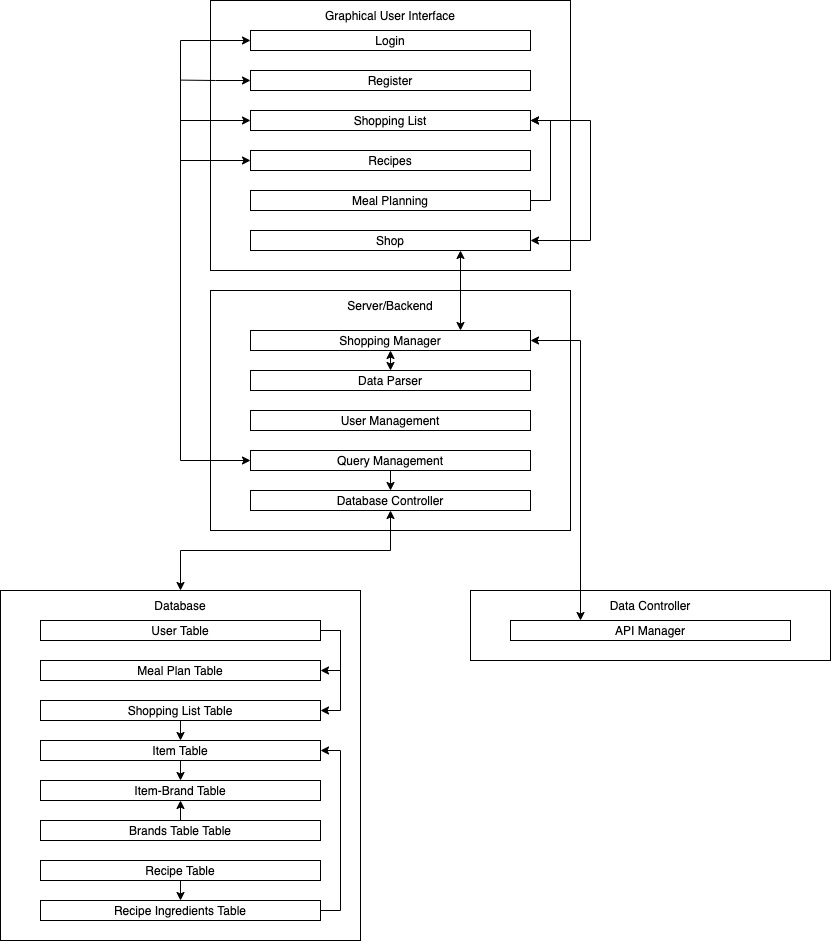
\includegraphics[width=0.90\textwidth]{images/flowChart}
 \caption{System architecture}
\end{figure}
